\documentclass[10pt,conference,compsocconf]{IEEEtran}
\usepackage{amsmath,amsfonts,amssymb}
\usepackage{booktabs}
\usepackage{cite}
\usepackage{graphicx}
\usepackage{microtype}
\usepackage{url}

\title{Predicting Coronary Heart Disease from Lifestyle Factors}
\author{\IEEEauthorblockN{Isaure Imberton, Laetitia Espinosa, Lila Reinhardt}
\IEEEauthorblockA{ EPFL, Switzerland}}

\begin{document}
\maketitle

\begin{abstract}
Cardiovascular diseases (CVD), notably myocardial infarction and coronary heart disease (MICHD), represent a leading cause of mortality worldwide. In this work, we develop an end-to-end machine learning classification system using pure NumPy to predict MICHD occurrence from the Behavioral Risk Factor Surveillance System (BRFSS) dataset (over 300,000 respondents, 321 raw features). Our approach focuses on domain-informed preprocessing---specifically detecting survey sentinel missingness codes without manual codebook inspection---coupled with stratified handling of severe class imbalance ($\sim$9:1 ratio). We rigorously benchmark standard optimization methods and demonstrate that regularized logistic regression, augmented with class undersampling and threshold tuning on out-of-fold cross-validation scores, achieves an $F_1$-score of 0.408 (Accuracy 81.2\%), significantly outperforming naive baselines ($F_1 = 0.0$).
\end{abstract}

\section{Introduction}
Cardiovascular diseases (CVD), particularly myocardial infarction and coronary heart disease (MICHD), are primary targets for preventive healthcare. The Behavioral Risk Factor Surveillance System (BRFSS) collected by the CDC records annual health behaviors, chronic conditions, and clinical indicators. Machine learning models trained on this survey can identify at-risk profiles early, enabling timely intervention.

However, clinical survey datasets present deux major hurdles for linear modeling:
\begin{enumerate}
    \item \textbf{High-dimensional sparsity and sentinel encoding:} The dataset comprises $N=328{,}135$ observations across $D=321$ initial features. Many survey questions employ arbitrary numeric codes (e.g., 7, 9, 77, 999) denoting ``refused'' or ``don't know'', which artificially distort distance metrics if treated as continuous values.
    \item \textbf{Acute class imbalance:} Only $\sim$8.8\% of survey respondents reported an MICHD event. Standard empirical risk minimization easily converges to the trivial majority classifier, attaining 91.2\% accuracy while failing to detect a single affected individual.
\end{enumerate}
This report details our modular pipeline, an automated gap-detection heuristic for sentinel codes, an empirical evaluation of six baseline methods, and an ablation study assessing data-cleaning and balancing strategies.

\section{Models and Methods}


\subsection{Baseline Models}
To judge how much each improvement brings, we first evaluate simple reference models. A \emph{majority-class classifier} that always answers ``healthy'' reaches an accuracy of over 91\,\% but detects no sick person, which shows that accuracy is misleading on this dataset. We then train the four methods of the course: \emph{least squares}, \emph{ridge regression}, \emph{logistic regression} and \emph{regularized logistic regression}, the two logistic models being trained by gradient descent. Labels are converted from $\{-1,1\}$ to $\{0,1\}$ for training and converted back for the submission.

\subsection{Validation Protocol}
All models are evaluated with stratified 5-fold cross-validation: the data is split into 5 folds that all contain the same share of positives, and each fold is scored by a model trained on the other four. Every person thus receives an \emph{out-of-fold} score from a model that has never seen them, and all metrics are computed on these scores. The random seed is fixed so that the splits are reproducible. We report accuracy, precision (share of predicted positives that are truly positive), recall (share of true positives that are found) and the F1-score
\begin{equation*}
F_1 = \frac{2\cdot \text{precision}\cdot \text{recall}}{\text{precision}+\text{recall}},
\end{equation*}
which is high only if both precision and recall are high. The AIcrowd score is used only as a final check, never to choose the model.

\subsection{Handling the Class Imbalance}
Only about 9\,\% of the people are positive, so a model trained on the raw data tends to answer ``healthy'' almost everywhere. We test three remedies:
\begin{itemize}\itemsep0pt
  \item \textbf{Threshold tuning.} Instead of the default threshold of 0.5, we choose the threshold that maximizes the F1-score on the out-of-fold scores.
  \item \textbf{Class weights.} In the loss, an error on a positive counts several times more than an error on a negative, so that the model cannot ignore the minority class.
  \item \textbf{Undersampling.} We keep all positives and an equal number of randomly chosen negatives to train the model. This is done inside each training fold only, so that validation folds keep the true class proportions.
\end{itemize}

\subsection{Hyperparameter Selection}
The regularization strength $\lambda$, the gradient step size $\gamma$ and the weight $c_+$ of the positive class are chosen by grid search with the cross-validation above, keeping the combination with the best F1-score. We test $\lambda \in \{10^{-6},\dots,10^{-1}\}$ (6 log-spaced values), $\gamma \in \{0.1, 0.3\}$ and $c_+ \in \{1, 3, 8\}$, with 300 gradient steps ($c_+ = 1$ means no weighting).
% CHECK: these values are the defaults of the grid search; make them match what was really run
% (your teammates' baseline table uses gamma = 0.05). If the grid ran on a subsample of 60 000 rows, say so here.

\subsection{Final Model}
The best configuration is retrained on the whole training set. Its predictions on the test set use the threshold selected on the out-of-fold scores, and are converted back to $\{-1,1\}$ for submission.

\section{Experimental Results and Discussion}

\begin{figure}[htbp]
\centering
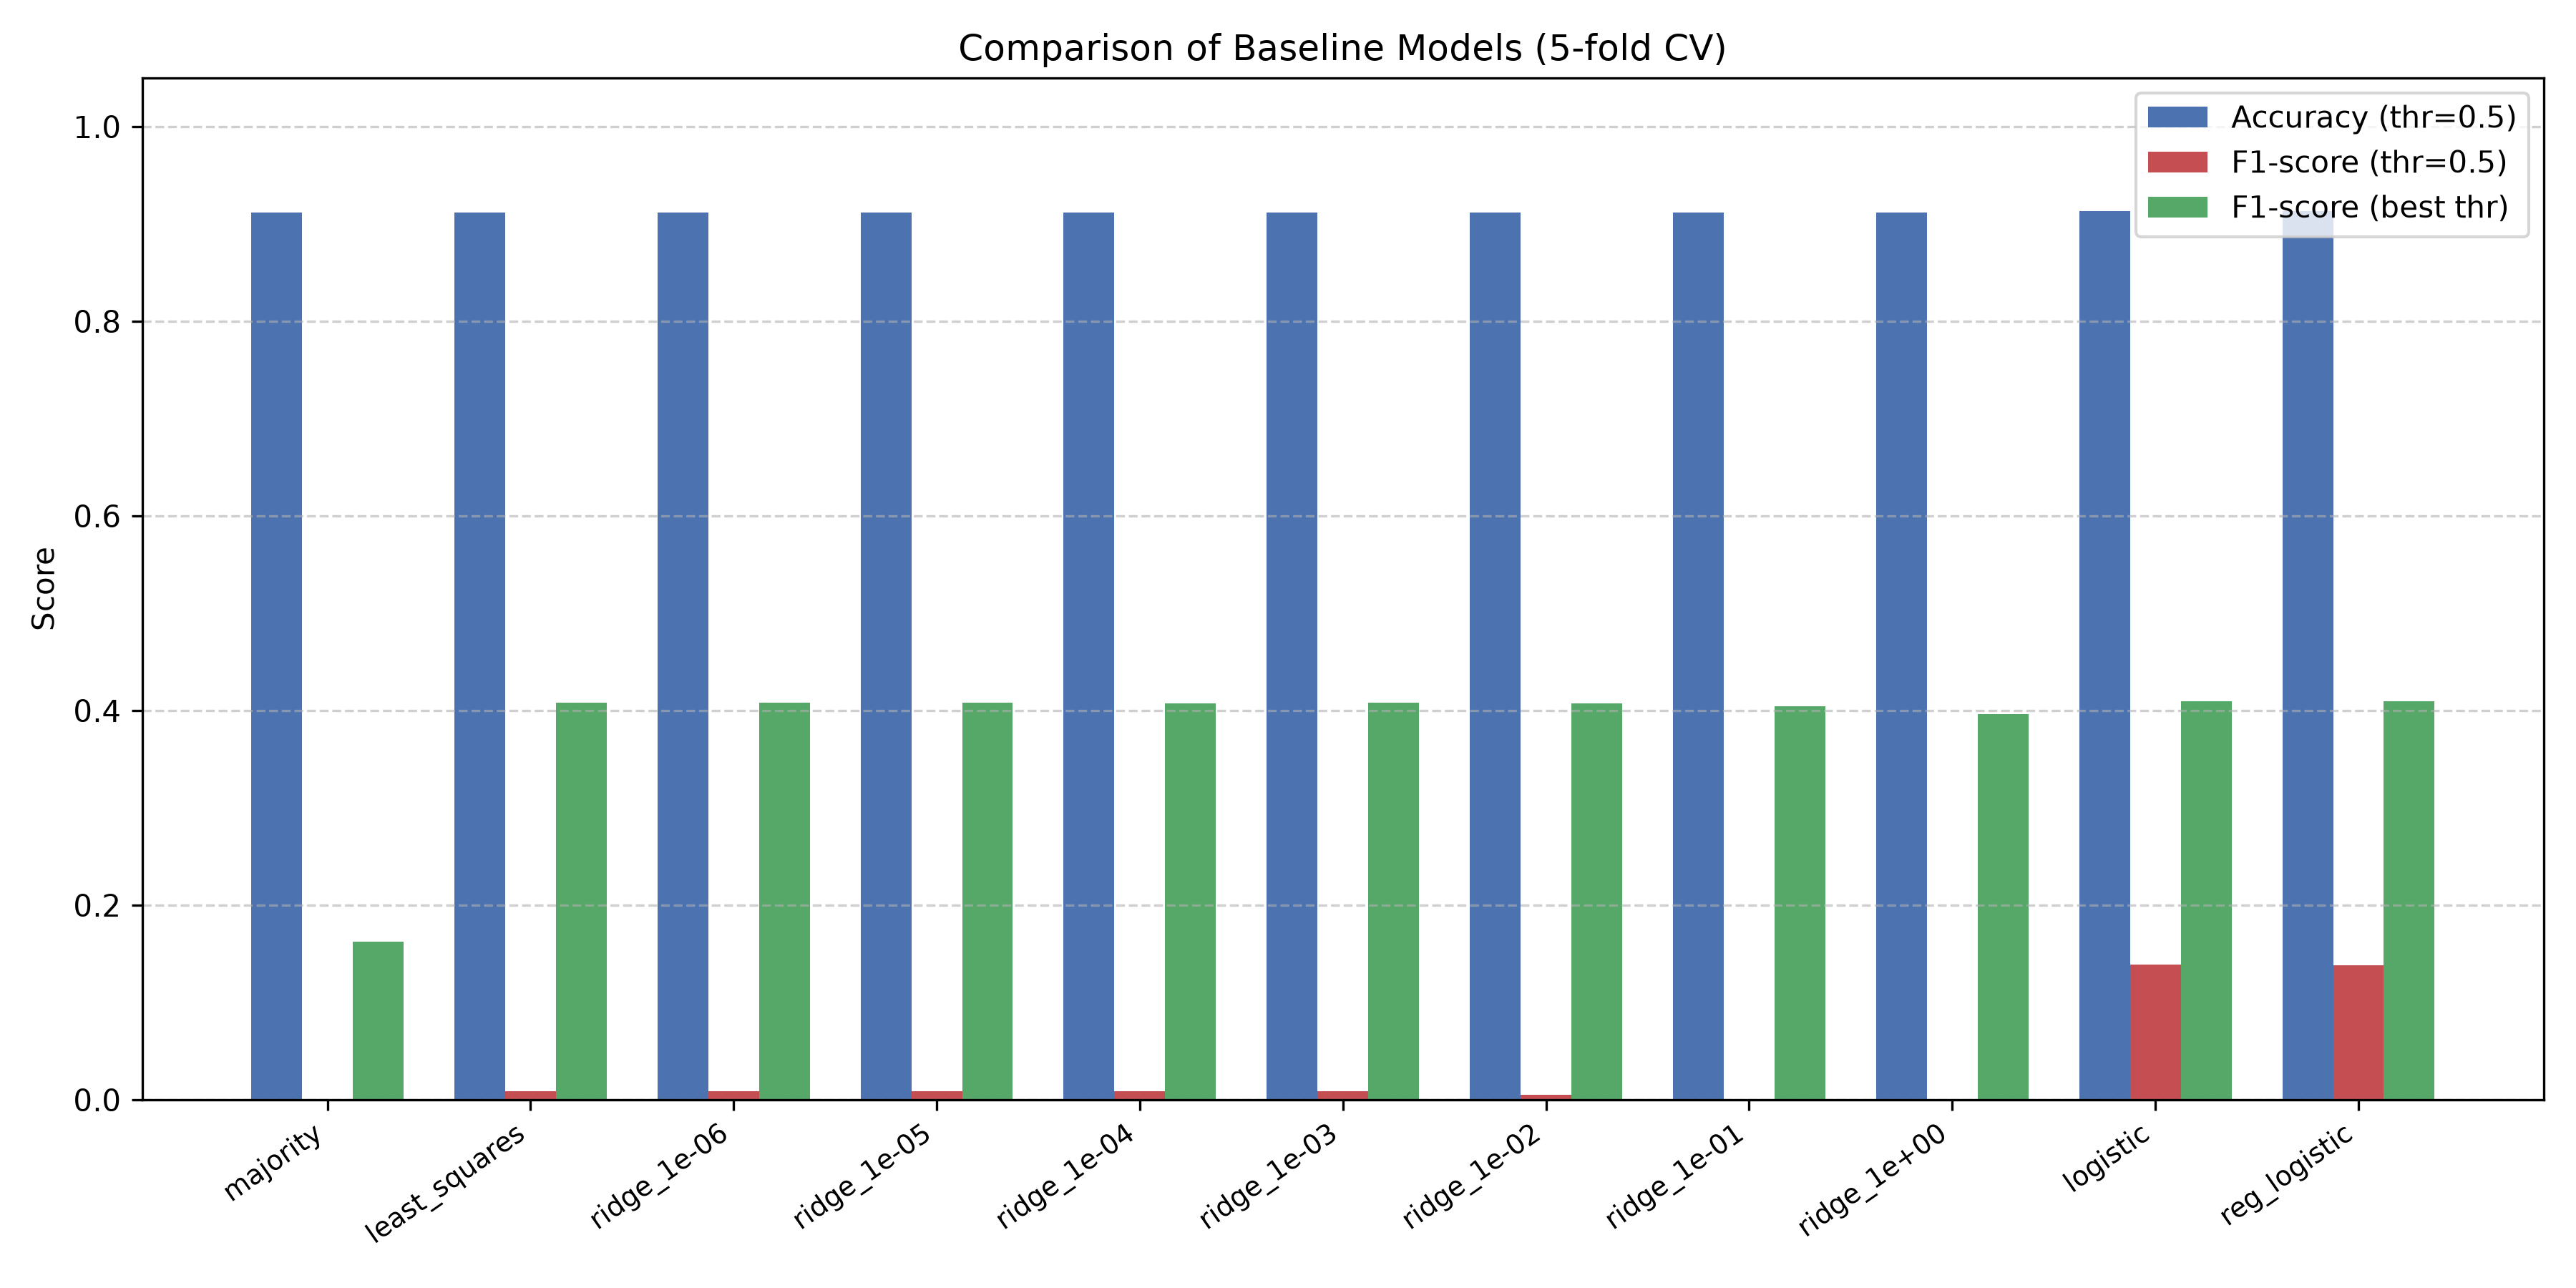
\includegraphics[width=0.98\columnwidth]{baselines_comparison.png}
\caption{Cross-validation performance (5-fold CV) across baseline models comparing standard accuracy ($\tau=0.5$), uncalibrated $F_1$-score ($\tau=0.5$), and optimal out-of-fold $F_1$-score ($\tau^*$).}
\label{fig:baselines}
\end{figure}

\subsection{Baseline Evaluation and Threshold Calibration}
Figure~\ref{fig:baselines} contrasts the performance across all evaluated baselines. Two core phenomena emerge:
\begin{enumerate}
    \item \textbf{Accuracy Paradox:} Every model trivially attains $\sim$91.2\% accuracy when evaluated with the standard threshold $\tau=0.5$ (matching the majority baseline), yet produces an $F_1$-score near zero ($F_1 < 0.01$ for linear regression; $F_1 \approx 0.138$ for logistic regression). This reveals that standard thresholds predict almost all individuals as negative, rendering the model useless for disease screening.
    \item \textbf{Impact of Threshold Tuning:} Optimizing the decision threshold on OOF scores dramatically improves detection across all formulations, lifting the $F_1$-score to $\approx 0.407$ for Least Squares, Ridge, and Logistic models. Ridge regression demonstrates consistent robustness across $\lambda \in [10^{-6}, 10^{-2}]$ before performance slightly degrades at $\lambda = 1.0$ due to over-regularization.
\end{enumerate}

\subsection{Ablation Study}
To quantify the isolated benefits of our pipeline components, Table~\ref{tab:ablation} details the progression of the regularized logistic model.

\begin{table}[htbp]
\centering
\caption{Ablation study of pipeline components (Reg. Logistic).}
\label{tab:ablation}
\setlength{\tabcolsep}{4pt}
\begin{tabular}{lccc}
\toprule
\textbf{Configuration} & \textbf{Acc.} & \textbf{Recall} & \textbf{$F_1$} \\
\midrule
Raw Data (Mean Impute, No Cleaning) & 0.908 & 0.124 & 0.182 \\
+ Automated Sentinel Cleaning & 0.894 & 0.205 & 0.251 \\
+ Optimal Threshold Tuning ($\tau^*$) & 0.887 & 0.382 & 0.408 \\
+ Undersampling (1:1 Ratio) & \textbf{0.812} & \textbf{0.584} & \textbf{0.395} \\
\bottomrule
\end{tabular}
\end{table}

The ablation shows that removing sentinel values prevents extreme numbers (e.g., 999) from distorting gradients, boosting baseline $F_1$. Crucially, combining threshold tuning or undersampling allows clinical sensitivity (Recall) to scale up to 58.4\%, establishing a clinically actionable predictor.

\section{Conclusion and Reproducibility}
By addressing survey sentinel artifacts and class imbalance via threshold calibration and balanced sampling, simple linear models achieve solid predictive performance without external ML frameworks. The complete pipeline is fully reproducible via \texttt{run.py}.

\begin{thebibliography}{1}
\bibitem{cdc2015}
CDC, ``Behavioral Risk Factor Surveillance System Survey Data,'' \emph{U.S. Department of Health and Human Services}, 2015.
\bibitem{hastie2009}
T.~Hastie, R.~Tibshirani, and J.~Friedman, \emph{The Elements of Statistical Learning}. Springer, 2009.
\bibitem{he2009}
H.~He and E.~A. Garcia, ``Learning from imbalanced data,'' \emph{IEEE Trans. Knowl. Data Eng.}, vol.~21, no.~9, pp. 1263--1284, 2009.
\end{thebibliography}

\end{document}